\section{September 26}

\subsection{Generalized NFA} \label{sec:GNFA}
\begin{definition}
  A Generalized NFA (GNFA) has transitions labeled with regular expressions. Can follow a transition by reading a matching block of input symbols.
\end{definition}
We can convert any GNFA into a "simple form":
\begin{enumerate}
  \item Accept state is unique. No transitions leaving accept state. Add new accept state, $\varepsilon$-transitions from old accept states to new one.

  \item No transitions entering the start state. 
  Add new start state, $\varepsilon$-transitions from new start states to old one.
  
  \item At most 1 transition between each pair of states. If multiple transitions between two nodes labeled $R_1 , R_2 , ...,$ replace with transition $ R_1 \cup R_2 \cup ...$
\end{enumerate}
\begin{theorem}
  A is Regular $\Rightarrow \: \exists $ reg. ex. R : A = L(R).
\end{theorem}
\begin{itemize}
  \item Start with DFA D that recognizes A.
  \item Convert it to GNFA G that has "simple form".
  \item \bf Remove intermediate states of G one at a time without changing which language it recognizes. 
  \begin{itemize}
    \item Remove state $q_{kill}$
    \item For each pair of states $q_i , \: q_j $ connected through $q_{kill}$ as shown, add a transition from $q_i \text{ to } \: q_j $ labeled with RE~.
    \item Continue to combine edges with $\cup$ until the GNFA is just a single RE~
  \end{itemize}
\end{itemize}

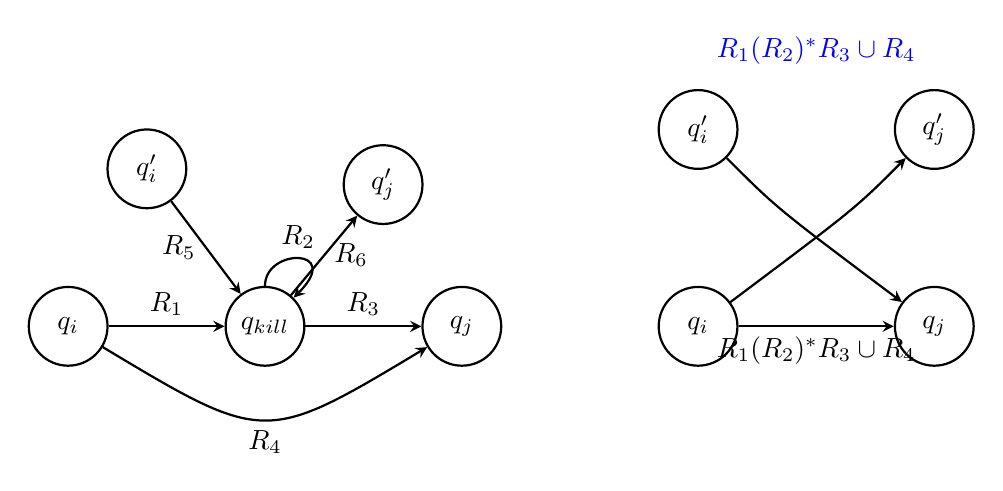
\begin{tikzpicture}[
    thick,
    >=stealth
]

% Left diagram
% States
\node[circle,draw,minimum size=1cm] (qi1) at (0,0) {$q_i$};
\node[circle,draw,minimum size=1cm] (qkill) at (2.5,0) {$q_{\text{kill}}$};
\node[circle,draw,minimum size=1cm] (qj1) at (5,0) {$q_j$};

% Top states
\node[circle,draw,minimum size=1cm] (qi_prime1) at (1,2) {$q'_i$};
\node[circle,draw,minimum size=1cm] (qj_prime1) at (4,1.8) {$q'_j$};

% Self-loop on qkill
\draw[->] (qkill) .. controls (2.5,1) and (3.5,1) .. node[above] {$R_2$} (qkill);

% Main transitions
\draw[->] (qi1) -- node[above] {$R_1$} (qkill);
\draw[->] (qkill) -- node[above] {$R_3$} (qj1);
\draw[->] (qi1) .. controls (2.5,-1.5) .. node[below] {$R_4$} (qj1);

% Top transitions
\draw[->] (qi_prime1) -- node[left] {$R_5$} (qkill);
\draw[->] (qkill) -- node[right] {$R_6$} (qj_prime1);

% Right diagram (simplified)
% States
\node[circle,draw,minimum size=1cm] (qi2) at (8,0) {$q_i$};
\node[circle,draw,minimum size=1cm] (qj2) at (11,0) {$q_j$};

% Top states
\node[circle,draw,minimum size=1cm] (qi_prime2) at (8,2.5) {$q'_i$};
\node[circle,draw,minimum size=1cm] (qj_prime2) at (11,2.5) {$q'_j$};

% Main transition with label
\draw[->] (qi2) -- node[below] {$R_1(R_2)^*R_3 \cup R_4$} (qj2);

% Curved arrows
\draw[->] (qi_prime2) .. controls (9,1.5) .. (qj2);
\draw[->] (qi2) .. controls (10,1.5) .. (qj_prime2);

% Title above right diagram
\node[text=blue] at (9.5,3.5) {$R_1(R_2)^*R_3 \cup R_4$};

\end{tikzpicture}

\newpage
Regular Expressions In Practice:
\begin{itemize}
  \item Used widely for pattern-matching, searching.
  \begin{itemize}
    \item Specify the format of a string such as a phone number, address, credit card number, license plate \dots
    \item Search a document to see if it contains some credit card number.
  \end{itemize}
  \item What algorithm is used: 
  \\ regex $\rightarrow$ NFA $\rightarrow$ DFA
\end{itemize}

\newpage
\subsection{Non-Regular Languages (Pumping Lemma)}
Not all languages are regular. Consider:
$L = \{ 0^n 1^n \: : \: n \geq 0 \} \:\:(\text{e.g. 0011} \in L \text{ but 001 } \notin L)$
\begin{theorem} \label{theo:pumping}
  Intuition: A DFA for L would need to remember how many 0's it has seen. Not enough memory
\end{theorem}
Our Plan:
\begin{itemize}
  \item Direct proof that $L = \{ 0^n 1^n \: : \: n \geq 0 \}$ is not regular
  \item Generalize the above ideas to "pumping lemma"
  \item Use "Pumping Lemma" to prove several other languages are not regular.
\end{itemize}
\begin{proof} \ref{theo:pumping}
  Assume by contradiction there is a DFA $M$ that recognized $L$. Let number of states in M = $p$.
  \\ Let $r_k \in Q$ be the state M reaches after reading $0^k$.
  \\ Then for some $0 \leq i \leq j \leq q$ we have $r_i = r_j$. 
  \\ M must accept $0^i 1^i \in L$.
  \\ $\Rightarrow$ M accepts $0^j 1^i \notin L$.
\end{proof}

\begin{lemma}
  Pumping Lemma:
  \\ If L is a regular language, then:
  \\ $\exists p \in \mathbb{Z}, p \geq 0$ (pumping length)
  \\ $\forall \text{strings }w \in L$ of length $|w| \geq P$
  \\ $\exists$ strings x,y,z $: w = xyz, |y| > 0, \: |xy| \leq p$
  \\ $\forall i \in \mathbb{N}, xy^iz \in L$.
\end{lemma}

To prove L is not regular, use contrapositive:
\begin{definition} \label{def:contrapositive}
  Contrapositive: $A \Rightarrow B = \neg B \Rightarrow \neg A$
\end{definition}
Recall De Morgan's law:
\begin{definition} \label{def:demorgan}
  $\neg \forall x \phi(x)$ is the same as
\end{definition}

\begin{figure}[htp]
  \centering
  \includegraphics[width=12cm]{"pumpinglemma.png"}
\end{figure}

\newpage
Recall that the pumping lemma requires you to give a strategy for winning the following game:
\begin{itemize}
  \item The adversary chooses some integer $p$.
  \item You choose a string $w \in L$ such that $|w| \geq p$.
  \item The adversary chooses strings $x,y,z$ such that $w = xyz$ and $|xy| \leq p, |y| \geq 1$.
  \item You choose an integer $i$ and you win if $xy^iz$ is not in $L$.
\end{itemize}
Therefore, for each language you ONLY need to answer the following questions (be concise):
\begin{enumerate}
  \item What's your strategy for choosing the string $w$ in the above game?
  \item What's your strategy for choosing  the integer $i$ in the above game?
  \item How do you know that $xy^iz$ is not in $L$? 
\end{enumerate}
To show L is not regular, show:
\begin{enumerate}
  \item $\forall p \in \mathbb{N}$
  \item $\exists \text{ strings } w \in L$ of length $|w| \geq P$
  \item $\forall \text{ strings } x,y,z \: : \: w = xyz, |y| > 0, |xy| \leq p$
  \item $\exists i \in \mathbb{N}, x y^i z \notin L$
\end{enumerate}